\section{Ход работы}

Пусть имеeтся база данных со схемой, изображенной на рисунке~\ref{pic:db_scheme}.

\begin{figure}[h]
  \centering
  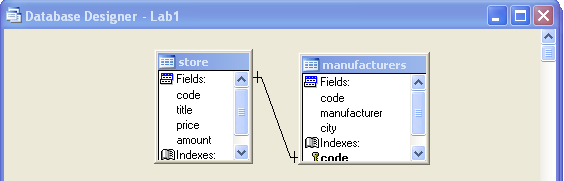
\includegraphics[width=0.5\linewidth]{structure}
  \caption{Схема базы данных\label{pic:db_scheme}}
\end{figure}

В этой базе данных имеются две таблицы (store и manufacturers) изображенные на рисунке~\ref{pic:db_content}.

\begin{figure}[h]
        \centering
        \begin{subfigure}[b]{0.7\textwidth}
                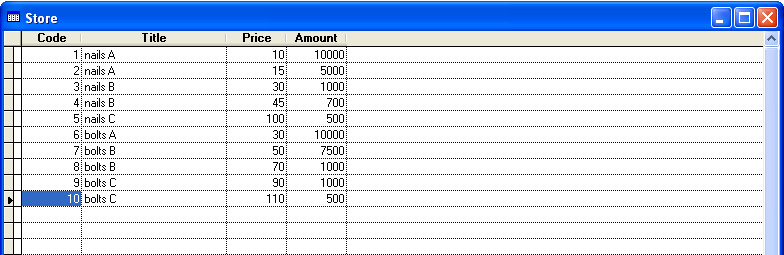
\includegraphics[width=\textwidth]{store}
                \caption{Таблица Store}
        \end{subfigure}

        \bigskip
        
        \begin{subfigure}[b]{0.7\textwidth}
                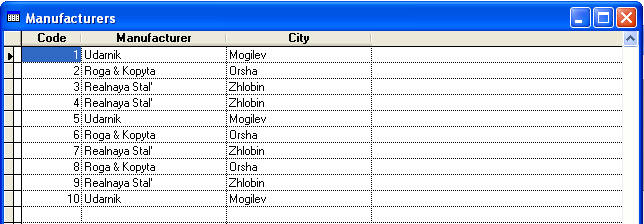
\includegraphics[width=\textwidth]{manufacturers}
                \caption{Таблица Manufacturers}
        \end{subfigure}
        \caption{Содержимое таблиц БД\label{pic:db_content}}
\end{figure}

Будем производить с ними операции в соответствии с заданием средствами языка SQL.

\subsection{Изменение записи}

Требуется изменить цену, название и количество товара
Название изменяемого товара ввести с экрана.

\begin{figure}[h!t]
    \center{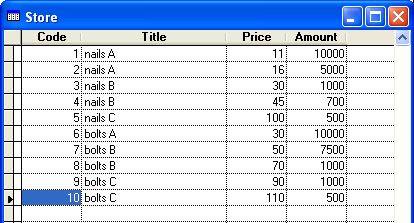
\includegraphics[width=0.7\linewidth]{1_1_update_price}}
  \caption{Результат увеличения цены на 10\% для товара с title=Nails A}
\end{figure}

\begin{lstlisting}[float,caption=Source code]
PROCEDURE 1_1_update_price
	i_title = "?"
	i_percent = 0

	@ 0,0 CLEAR
	@ 1,1 CLEAR to 1,50
	@ 1,1 SAY "title = " GET i_title size 1,20
	READ
	
	@ 1,1 CLEAR to 1,50
	@ 1,1 SAY "percent = " GET i_percent size 1,6
	READ
	
	UPDATE store SET price = price * (1 + i_percent / 100) WHERE title = i_title
	BROWSE
ENDPROC
\end{lstlisting}

\begin{figure}[h!t]
    \center{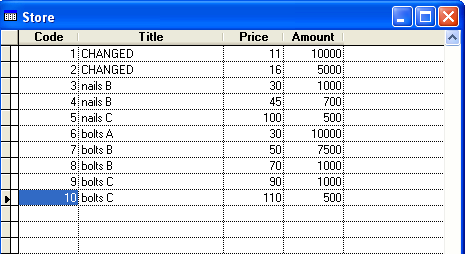
\includegraphics[width=0.7\linewidth]{1_2_update_title}}
  \caption{Результат изменения title для товара с title=Nails A на title=CHANGED}
\end{figure}

\begin{lstlisting}[float,caption=Source code]
PROCEDURE 1_2_update_title
	old_title = "?"
	new_title = "?"

	@ 0,0 CLEAR
	@ 1,1 CLEAR to 1,50
	@ 1,1 SAY "title = " GET old_title size 1,20
	READ
	
	
	@ 1,1 CLEAR to 1,50
	@ 1,1 SAY "new title = " GET new_title size 1,20
	READ
	
	UPDATE store SET title = new_title WHERE title = old_title
	BROWSE
ENDPROC
\end{lstlisting}

\begin{figure}[h!t]
    \center{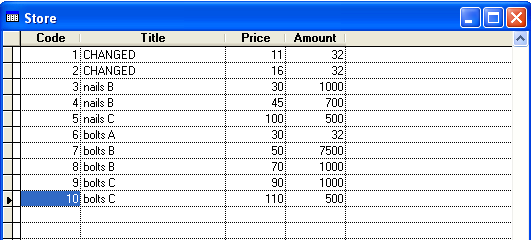
\includegraphics[width=0.7\linewidth]{1_3_update_amount}}
  \caption{Результат изменения количества товара с title=CHANGED}
\end{figure}

\begin{lstlisting}[float,caption=Source code]
  PROCEDURE 1_3_update_amount
	i_title = "?"
	i_amount = 0

	@ 0,0 CLEAR
	@ 1,1 CLEAR to 1,50
	@ 1,1 SAY "title = " GET i_title size 1,20
	READ
	
	@ 1,1 CLEAR to 1,50
	@ 1,1 SAY "new amount = " GET i_amount size 1,6
	READ
	
	UPDATE store SET amount = i_amount WHERE title = i_title
	BROWSE
  ENDPROC
\end{lstlisting}

\subsection{Вывод количества товара данного наименования}
\addcontentsline{toc}{subsection}{Вывод количества товара данного наименования}

\begin{figure}[h!t]
    \center{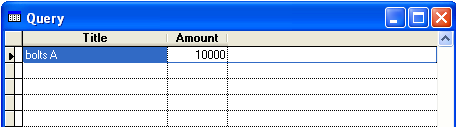
\includegraphics[width=0.7\linewidth]{2_select_amount_with_current_title}}
  \caption{Результат вывода количества товара с title=bolts A}
\end{figure}

\begin{lstlisting}[float,caption=Source code]
  PROCEDURE 2_select_amount_with_current_title
	i_title = "?"

	@ 0,0 CLEAR
	@ 1,1 CLEAR to 1,50
	@ 1,1 SAY "title = " GET i_title size 1,20
	READ
	
	SELECT title, amount FROM store WHERE title = i_title
  ENDPROC
\end{lstlisting}


\subsection{Вывод названия и цены товара с сортировкой названия товара алфавиту}
\addcontentsline{toc}{subsection}{Вывод названия и цены товара с сортировкой названия товара алфавиту}

\begin{figure}[h!t]
    \center{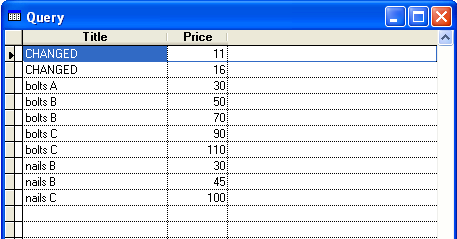
\includegraphics[width=0.7\linewidth]{3_select_sorted_title_price}}
  \caption{Результат вывода названия и цены товара с сортировкой названия товара по алфавиту}
\end{figure}

\begin{lstlisting}[float,caption=Source code]
PROCEDURE 3_select_sorted_title_price
	SELECT title, price FROM store ORDER BY title
ENDPROC
\end{lstlisting}

\subsection{Вывод названия товара и выручки как вычисляемого поле=цена*количество}
\addcontentsline{toc}{subsection}{Вывод названия товара и выручки как вычисляемого поле=цена*количество}

\begin{figure}[h!t]
    \center{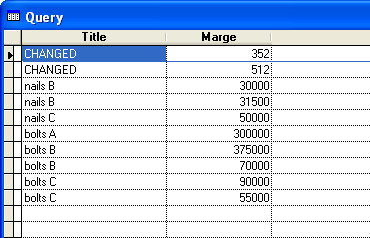
\includegraphics[width=0.7\linewidth]{4_select_title_marge}}
  \caption{Результат вывода названия товара и выручки как вычисляемого marge=price*amount}
\end{figure}

\begin{lstlisting}[float,caption=Source code]
PROCEDURE 4_select_title_marge
	SELECT title, price*amount AS marge FROM store
ENDPROC
\end{lstlisting}

\subsection{Вывод названия товара с минимальной ценой с отображением цены}
\addcontentsline{toc}{subsection}{Вывод названия товара с минимальной ценой с отображением цены}

\begin{figure}[h!t]
    \center{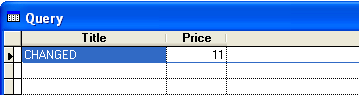
\includegraphics[width=0.7\linewidth]{5_select_title_with_min_price}}
  \caption{Результат вывода названия товара с минимальной ценой с отображением цены}
\end{figure}

\begin{lstlisting}[float,caption=Source code]
PROCEDURE 5_select_title_with_min_price
	SELECT title, price FROM store ;
	WHERE price IN (SELECT MIN(price) FROM store)
ENDPROC
\end{lstlisting}

\subsection{Вывод названия товара, цены, фирмы и ее адреса}
\addcontentsline{toc}{subsection}{Вывод названия товара, цены, фирмы и ее адреса}

\begin{figure}[h!t]
    \center{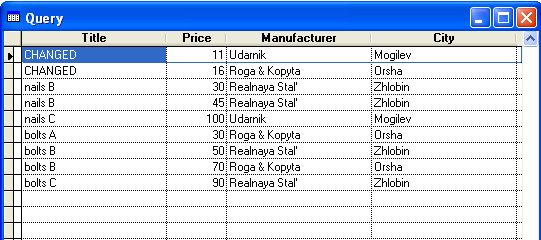
\includegraphics[width=0.7\linewidth]{6_select_title_price_manufacturer_city}}
  \caption{Результат вывода названия товара, цены, фирмы и ее адреса}
\end{figure}

\begin{lstlisting}[float,caption=Source code]
PROCEDURE 6_select_title_price_manufacturer_city
	SELECT store.title, store.price, manufacturers.manufacturer, manufacturers.city FROM ;
	store INNER JOIN manufacturers ON ;
	store.code = manufacturers.code 
ENDPROC
\end{lstlisting}

\subsection{Вывод названия фирмы, производящей самый дешевый товар}
\addcontentsline{toc}{subsection}{Вывод названия фирмы, производящей самый дешевый товар}

\begin{figure}[h!t]
    \center{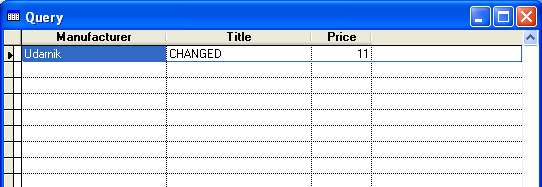
\includegraphics[width=0.7\linewidth]{7_select_manufacturer_min_price}}
  \caption{Результат вывода названия фирмы, производящей самый дешевый товар}
\end{figure}

\begin{lstlisting}[float,caption=Source code]
PROCEDURE 7_select_manufacturer_min_price
	SELECT manufacturers.manufacturer, store.title, store.price FROM ;
	store INNER JOIN manufacturers ON ;
	store.code = manufacturers.code ;
	WHERE store.price IN (SELECT MIN(price) FROM store)
ENDPROC
\end{lstlisting}

\subsection{Примеры работы SELECT ... GROUP BY c группированием}
\addcontentsline{toc}{subsection}{Припмеры работы SELECT ... GROUP BY c группированием}

\begin{figure}[h!t]
    \center{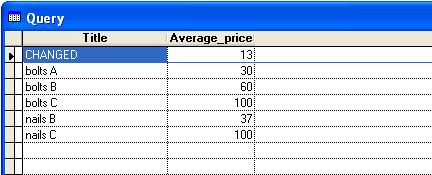
\includegraphics[width=0.7\linewidth]{8_1_select_avg_price_group_by_title}}
    \caption{Результат вывода средней стоимости товаров с группировкой по названию}
\end{figure}

\begin{lstlisting}[float,caption=Source code]
PROCEDURE 8_1_select_avg_price_group_by_title
	SELECT title, AVG(price) AS average_price FROM store ;
	GROUP BY title
ENDPROC
\end{lstlisting}


\begin{figure}[h!t]
    \center{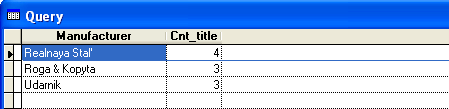
\includegraphics[width=0.7\linewidth]{8_2_select_title_count_by_manufacturers}}
  \caption{Результат вывода количества видов выпускаемой продукции, сгрупированной по производителям}
\end{figure}

\begin{lstlisting}[float,caption=Source code]
PROCEDURE 8_2_select_titles_count_by_manufacturers
	SELECT manufacturer, COUNT(title) FROM manufacturers ;
	GROUP BY manufacturer
ENDPROC
\end{lstlisting}

\subsection{Вывод названия фирмы, продающей товар по самой низкой цене}
\addcontentsline{toc}{subsection}{Вывод названия фирмы, продающей товар по самой низкой цене}

Название товара ввести с экрана. В нашем случае название товара = nails B.
\begin{figure}[h!t]
    \center{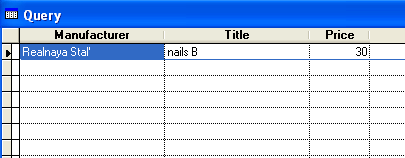
\includegraphics[width=0.7\linewidth]{9_select_manufacturer_with_minimal_price_by_title}}
  \caption{Результат вывода названия фирмы, продающей товар по самой низкой цене при title=nails C}
\end{figure}

\begin{lstlisting}[float,caption=Source code]
PROCEDURE 9_select_manufacturer_with_minimal_price_by_title
	i_title = "?"

	@ 0,0 CLEAR
	@ 1,1 CLEAR to 1,50
	@ 1,1 SAY "title = " GET i_title size 1,20
	READ
	
	SELECT manufacturers.manufacturer, store.title, store.price FROM ;
	store INNER JOIN manufacturers ON ;
	store.code = manufacturers.code ;
	WHERE store.price IN (SELECT MIN(price) FROM store WHERE store.title = i_title) AND store.title = i_title
ENDPROC
\end{lstlisting}

\subsection{Демонстрация использования курсора}
\addcontentsline{toc}{subsection}{Демонстрация использования курсора}

\begin{figure}[h!t]
    \center{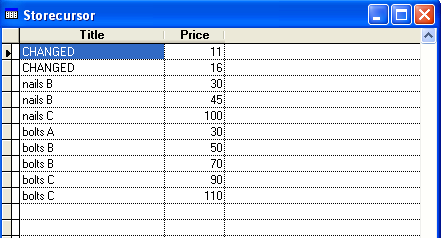
\includegraphics[width=0.7\linewidth]{10_usage_cursor}}
  \caption{Использование курсора}
\end{figure}

\begin{lstlisting}[float,caption=Source code]
PROCEDURE 10_usage_cursor
	SELECT title, price FROM store ;
	INTO CURSOR storeCursor NOFILTER
	
	BROWSE
ENDPROC
\end{lstlisting}


\subsection{Демонстрация работы представления}
\addcontentsline{toc}{subsection}{Демонстрация работы представления}

\begin{figure}[h!t]
    \center{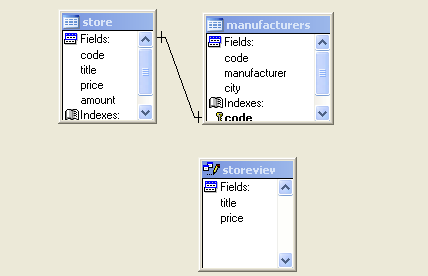
\includegraphics[width=0.7\linewidth]{11_usage_view}}
  \caption{Использование представления}
\end{figure}

\begin{lstlisting}[float,caption=Source code]
PROCEDURE 11_usage_view
	CREATE SQL VIEW storeView ;
	AS SELECT title, price from STORE
ENDPROC
\end{lstlisting}


\subsection{Вывод таблицы через SELECT с вычисляемым полем НАЛОГ}
\addcontentsline{toc}{subsection}{Вывод таблицы через SELECT с вычисляемым полем НАЛОГ}

  Для вычисления налога использовать функцию IIF (налог считать так: если выручка от
  продажи товара больше 10 000, то налог равен 20\% от выручки, иначе – 13\% от
  выручки.

  \begin{figure}[h!t]
    \center{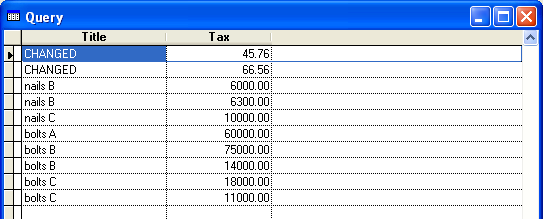
\includegraphics[width=0.7\linewidth]{12_select_with_tax}}
    \caption{Результат работы процедуры}
  \end{figure}

\begin{lstlisting}[float,caption=Source code]
PROCEDURE 12_select_with_tax
	SELECT title, IIF(price*amount<=10000, price*amount*0.13, price*amount*0.2) AS tax FROM store
ENDPROC
\end{lstlisting}
